
% !TEX encoding = UTF-8 Unicode
\documentclass[a4paper,11pt]{article}
\usepackage[francais]{babel}		% typographie franaise (french marche aussi)
%\usepackage[mac]{inputenc}		% lettres accentuées
\usepackage{color}
\usepackage[utf8]{inputenc}
\usepackage{graphicx, amsmath, amssymb}

\setlength{\textheight}{27cm}
\setlength{\topmargin}{-25mm}
\setlength{\textwidth}{18cm}
\setlength{\oddsidemargin}{-10mm} % marge gauche (im)paire = 1in. + x1mm
%\setlength{\evensidemargin}{0mm} % book : marge gauche paire = 1in. + x2mm
\setlength{\parskip}{1.2ex plus 0.9ex minus 0.4ex}

\newcommand{\dd} {\textrm d}   
\newcommand{\im} {\mathrm i}   
\newcommand{\e}  {\textrm e}   
\newcommand{\dpa}[2]  {\frac {\partial #1} {\partial #2}}   
\newcommand{\ddpa}[2] {\frac {\partial^{2} #1} {\partial #2 ^{2}}}   
\newcommand{\dto}[2]  {\frac {{\textrm d} #1} {{\textrm d} #2}}   
\newcommand{\ddto}[2] {\frac {\textrm{d}^{2} #1} {\textrm{d} #2 ^{2}}}

%-----------------------------------------------------------------------
\begin{document}
{\Large
\noindent
%M2R DET,

\begin{center}
{\bf Examen du cours d'instabilités, M2 DET \\
 4 février 2021} \\
{\it \small Durée 2 heures. La qualité de la présentation de la copie sera prise en compte. 
%Barme indicatif : I : 3 points, II 5 points, III : 12 points. %Présentation : 2 points.
} \\
{\it \small Documents autorisés : tous documents manuscrits ou imprimés.}
\end{center}

%{\it ELEMENTS DE CORRECTION}


}



%\newcommand{\rep}[1]{ {\em Réponse : #1 } }
\newcommand{\rep}[1]{  }
%\medskip
%-----------------------------------------------------------------------
%\textbf{I. Questions de cours}
%

\section{Effet de la compressibilité sur les propriétés de stabilité d'un écoulement de Poiseuille plan}

On a vu en cours les propriétés de stabilité de l'écoulement de Couette plan, considéré comme prototype des écoulements de "classe B", stables vis-à-vis des critères classiques non-visqueux mais affectés par l'instabilité de Tollmien-Schlishting.

Dans ce problème on souhaite étudier l'effet de la compressibilité sur ces instabilités.

On partira des équations de Navier-Stokes {\em compressibles } pour un fluide Newtonien, écrites sous la forme suivante :

$$
\frac{\partial \rho}{\partial t} + \vec{u} \cdot \vec{\nabla} \rho + \rho div ( \vec{u} ) = 0.
$$

$$
\rho \left[ \frac{\partial \vec{u}}{\partial t} + (\vec{u} \cdot \vec{\nabla}) \vec{u} \right] = - \vec{\nabla} p + \mu \Delta  \vec{u}
$$

On négligera les transferts thermiques au sein du fluide, ce qui permet de faire l'hypothèse d'un comportement adiabatique,
c.a.d. que la pression et la masse volumique sont reliés par une équation de Laplace : 

$$
p \rho^{-\gamma} = Cte. \qquad (\gamma = 1.4) 
$$
 
La solution de base correspond à une masse volumique $\rho_0$ et une pression $P_0$ constantes, ainsi qu'un champ de vitesse 
$\bar{U}(y) = U_m \left( 1 - \frac{y^2}{2 H^2} \right)$ où $U_m$ est la vitesse maximale, $H$ la demi-largeur du canal. 
 
Dans la suite on adimensionalisera les équations en posant $H \equiv 1,U_m \equiv 1, \rho_0 \equiv 1$. On pourra donc identifier $\bar{U}(y)$ 
avec sa version adimensionnelle (c.a.d. $\bar{U}(y) \equiv (1-y^2)$), et 
remplacer la viscosité par $\mu \equiv Re^{-1}$ où $Re = \rho_0 U_m H/\mu$ est le nombre de Reynolds.
 
 
\subsection{ Etablissement des équations linéarisées } 

On considère des petites perturbations par rapport à l'état de référence défini précédemment, sous la forme suivante :

$$
\vec{u} = \left[ \begin{array}{c} \bar{U}(y) \\ 0  \end{array} \right] + \left[ \begin{array}{c} u' \\ v'  \end{array} \right] ;
\quad p = P_0 + p', \quad  \rho = \rho_0 + \rho'.
$$

%Ici $\bar{U}(y) = U_m \left( 1 - \frac{y^2}{2 H^2} \right)$ est le profil de vitesse du "champ de base", $U_m$ la vitesse maximale, $H$ la demi-largeur du domaine. $P_0$ et $\rho_0$ sont considérés comme constants.

\begin{enumerate}
  \item Justifiez que sous l'hypothèse adiabatique $p'$ et $\rho'$ sont liés par:
  $$ p' = c_0^2 \rho', \qquad \mbox{ avec }  c_0^2 = \frac{\gamma P_0}{\rho_0}$$ 
  
  \rep{ 
  On écrit $$(P_0+p') (\rho_0 + \rho')^{-\gamma} = cte = P_0 \rho_0^{-\gamma}$$ 
  ou encore $$\left(1+\frac{p'}{P_0} \right) \left(1+\frac{\rho'}{\rho_0} \right)^{-\gamma} = 1 $$ 
  En linéarisant ceci conduit à $\frac{p'}{P_0} - \gamma \frac{\rho'}{\rho_0}  = 0$ d'où le résultat.
  }
  
 
  
  

Dans la suite, compte tenu du choix d'adimensionalisation, on pourra remplacer partout la vitesse du son par
$c_0 \equiv Ma^{-1}$ où $Ma = U_M/c_0$ est le nombre de Mach basé sur la vitesse maximale.

\item En linéarisant les équations de Navier-Stokes compressibles, 
donnez le système d'équations aux dérivées partielles linéaires gouvernant l'évolution des petites perturbations $[u',v',\rho']$. 

\rep{ 

Réécrivons les eqs de Navier-Stokes en détaillant les composantes :

$$
\frac{\partial \rho}{\partial t} + u \partial_x \rho +v \partial_y \rho + \rho (\partial_x u + \partial_y v)   = 0.
$$

$$
\rho \left[ \frac{\partial u}{\partial t} + u \partial_x u + v \partial_y u \right] = - \partial_x p + \mu  (\partial_{xx} u + \partial_{yy} u )
$$

$$
\rho \left[ \frac{\partial v}{\partial t} + u \partial_x v + v \partial_y v \right] = - \partial_y p + \mu  (\partial_{xx} v + \partial_{yy} v )
$$

On injecte le développement, et on néglige tous les termes non linéaires (de la forme $u' \times u', u' \times \rho'$, etc...)
On arrive à :

$$
\frac{\partial \rho'}{\partial t} + \bar{U}  \partial_x \rho'  + \rho_0 (\partial_x u' + \partial_y v')   = 0.
$$

$$
\rho_0 \left[ \frac{\partial u'}{\partial t} + \bar{U} \partial_x u' + v' \partial_y \bar{U} \right] = - \partial_x p' + \mu  (\partial_{xx} u' + \partial_{yy} u' )
$$

$$
\rho_0 \left[ \frac{\partial v'}{\partial t} + \bar{U} \partial_x v'  \right] = - \partial_y p' + \mu  (\partial_{xx} v' + \partial_{yy} v' )
$$
}


\item On recherche des solutions sous la forme de modes propres : 
$[u',v',\rho',p'] = Re \left( [\hat{u},\hat{v},\hat{\rho},\hat{p}] e^{i k x} e^{\lambda t} \right)$. 
Justifiez que $\lambda_r = Re(\lambda)$ correspond au taux de croissance de l'instabilité et que $c_r = - Im(\lambda)/k$ 
correspond à la vitesse de phase des modes correspondants.

\rep{ Les perturbations peuvent se mettre sous la forme 
$[u',v',\rho',p'] = Re \left( [\hat{u},\hat{v},\hat{\rho},\hat{p}] e^{i k (x-c_r t)} e^{\lambda_r t} \right)$. 
On reconnait une "onde" qui se propage à la vitesse $c_r$  tout en étant amplifiée exponentiellement.
}



\item 
Montrez que les équations écrites précédemment conduisent à :

%\begin{eqnarray}
%\rho_0 (\lambda +i k \bar{U}) \hat{u} + (\partial_y \bar{U}) \hat{v} &=&   - i k \hat{p} + \mu ( \partial_{yy} - k^2) \hat{u}, 
%\\
%\rho_0 (\lambda + i k \bar{U}) \hat{v} &=& - \partial_y \hat{p} + \mu ( \partial_{yy} - k^2) \hat{v}, 
%\\
%(c_0)^{-2} (\lambda + i k \bar{U})  \hat{p} &=&  - \rho_0 (i k  \hat{u} + \partial_y \hat{v})
%\end{eqnarray}

\begin{eqnarray}
(\lambda +i k \bar{U}) \hat{u} + (\partial_y \bar{U}) \hat{v} &=&   - i k \hat{p} + Re^{-1} ( \partial_{yy} - k^2) \hat{u}, 
\\
(\lambda + i k \bar{U}) \hat{v} &=& - \partial_y \hat{p} + Re^{-1}  ( \partial_{yy} - k^2) \hat{v}, 
\\
Ma^2 (\lambda + i k \bar{U})  \hat{p} &=&  - (i k  \hat{u} + \partial_y \hat{v})
\end{eqnarray}


\rep{ On remplace $\partial_x$ par $ik$, on utilise l'adimensionalisation indiquée, et on exprime $\hat{\rho}$ en fonction de $\hat{p}$ pour aboutir au résultat.}


%\item Montrez qu'avec une adimensionalisation adaptée, on arrive finalement à une expression matricielle sous la forme suivante:

%\begin{equation}
%\lambda  {\mathcal B} \, \hat{q} = {\mathcal A} \, \hat{q}
%\end{equation}
%avec  
%$$
%{\mathcal B} = 
%\left[
%\begin{array}{ccc} 
%1 & 0 & 0 \\ 
%0 & 1 & 0 \\
%0 & 0 & M^2  
%\end{array} 
%\right] 
%$$
%
%$$
%{\mathcal A} = 
%\left[
%\begin{array}{ccc} 
%-i k \bar{U} + Re^{-1} ( \partial_y^2 - k^2) & - \partial_y \bar{U} & - i k \\ 
%0 & -i k \bar{U} + Re^{-1} ( \partial_y^2 - k^2) & - \partial_y \\
%-i k  & -\partial_y  & -i k M^2 \bar{U}
%\end{array} 
%\right] 
%$$

%où apparaissent les nombres sans dimension $Re,M$ définis par
% $$
% Re = \frac{\mu}{\rho U_M H}; \quad M = \frac{U_M}{c_0}
% $$ 
% et où $\bar{U}(y)$  a été remplacé par sa version adimensionnelle : $\bar{U}(y)  \equiv (1-y^2)$.

%\item $^*$ {\em (Question hors-barème).} Montrez que dans le cas non visqueux ($Re^{-1} = 0$), on peut combiner les 3 équations linéaires pour exprimer $\hat{u}$ et $\hat{p}$ en fonction de $\hat{v}$, pour finalement arriver à une équation unique gouvernant $\hat{v}$, avec la forme suivante :
%$$
%\left[ \frac{ (\bar{U}-c) \hat{v}' - \bar{U}' \hat{v} }{1 - Ma^2 ( \bar{U}-c)^2} \right]' - k^2 (\bar{U}-c) \hat{v} =0
%$$
%(on a posé $c = i \lambda/k$).
%
%
%\item $^*$ {\em (Question hors-barème).} Que devient l'expression précédente lorsque $M\rightarrow 0$ ? Que reconnaissez-vous ?

%\subsection{Résolution numérique du problème}

\item Montrez que le problème peut se mettre sous la forme suivante:

\begin{equation}
\lambda  {\mathcal B} \, \hat{q} = {\mathcal A} \, \hat{q}
\end{equation}

où $ {\mathcal B}$ et  ${\mathcal A}$ sont des opérateurs à structure matricielle dont on donnera l'expression.
\rep{
$$
{\mathcal B} = 
\left[
\begin{array}{ccc} 
1 & 0 & 0 \\ 
0 & 1 & 0 \\
0 & 0 & M^2  
\end{array} 
\right] 
$$

$$
{\mathcal A} = 
\left[
\begin{array}{ccc} 
-i k \bar{U} + Re^{-1} ( \partial_y^2 - k^2) & - \partial_y \bar{U} & - i k \\ 
0 & -i k \bar{U} + Re^{-1} ( \partial_y^2 - k^2) & - \partial_y \\
-i k  & -\partial_y  & -i k M^2 \bar{U}
\end{array} 
\right] 
$$
}

\item Que constate-t-on pour $Ma=0$ ?

\rep{ On retombe sur le cas incompressible vu en cours.}

%\item Proposez la structure d'un programme pour résoudre numériquement ce problème aux valeurs propres. Expliquez notamment la méthode de construction des matrices, et le traitement des conditions limites sur les frontières du domaine.



%\item Expliquez la démarche permettant de résoudre numériquement le problème aux valeurs propres écrit précédemment. Détaillez en particulier le traitement des conditions limites dans la construction des matrices.



\subsection{ Interprétation des résultats  }

Un programme permettant de résoudre le problème a été écrit sur la base du projet EasyStab. Celui-ci a produit les résultats présentés dans les figures 1 à 3.

\item La figure 1 représente le spectre (ensemble des valeurs propres $\lambda$ complexes) pour le choix de paramètres ($Re = 10^4, Ma=0.1$, $k=1$). Discutez les résultats au vu du cas incompressible vu en cours. Quelles sont les ressemblances et différences ? Comment interpréter l'existence de modes caractérisés par des grandes valeurs de la vitesse de phase ($|c_r| = \mathcal{O} (10)$) ?

\rep{ Dans la région définie par $c_r\in [0,1]$ on reconnait des résultats similaires a ceux du cas incompressible vu en cours. En particulier il existe un unique mode instable, c'est l'onde de Tollmien-Schlishting. 

Les modes tels que $c_r = \mathcal{O}(10)$ correspondent, dimensionnellement, à $c_r = \mathcal{O}(c_0)$ vu que $c_0 \equiv 1/Ma = 10$.
On peut effectivement s'attendre à l'existence d'une famille de modes ayant ces propriétés : il s'agit d'ondes acoustiques se propageant dans le canal et qui sont faiblement amorties par la viscosité. Avec $M=0.1$ ces ondes acoustiques sont peu affectées par l'écoulement dans le canal.


 }


\item La figure 2$(a)$ représente la structure du mode le plus instable pour les paramètres précédents. Justifiez que ce mode possède une couche critique et donnez la position $y_c$ correspondante (ou les positions correspondantes). Qu'observe-t-on dans la structure du mode à cette position ? 

\rep{ On reconnait l'onde de Tollmien Schlishting. Avec l'adimensionalisation choisie la condition $c_r = U(y_c)$ s'écrit $c_r = (1-y_c^2)$ et conduit à $y_c \approx \pm 0.87$. On identifie en effet un comportement irrégulier du mode à cette position (indiquée par un pointillé sur la figure).}



\item La figure 3 représente le taux de croissance et la vitesse de phase du mode le plus instable en fonction de $k$ pour $Re = 10 000$, avec $M = 0.1$, $M=0.6$ et $M=2$. Que peut-on en conclure sur l'effet de la compressibilité sur les propriétés de stabilité de l'écoulement ?

\rep{ Les résultats pour  $M=0.1$ sont quasiment identiques aux résultats du cas incompressible. donc pour $M < 0.1$ la compressibilite n'a quasiment aucun effet sur l'instabilité de Tollmien Schlichting (correspondant à la bosse observée pour $k\approx 1$).
Lorsque $M$ augmente, on constate que la compressibilité a pour effet de restabiliser le mode de Tollmien Schlichting (le taux d'amplification maximal et la largeur de la bosse diminuent).  
Le second effet de la	 compressibilité est de conduite à l'apparitionn d'un nouveau mode instable qui n'existait pas dans le cas incompressible. Ce mode correspond à la seconde "bosse" pour $k\approx 2.6$.
}


\item La figure $2(b)$ représente la structure du mode le plus instable obtenu pour les paramètres $Re = 10^4, Ma = 2, k=2.6$. Comment peut-on comprendre physiquement la structure de ce mode ?

\rep{La structure du champ de vitesse montre des alternances de région de compression et de dilatation, décalées d'un quart de longueur d'onde avec les maximums et minimums de pression. On reconnait la structure caractéristique d'une onde acoustique. On constate que ce mode possède une couche critique. L'explication est donc que lorsque $M>1$ , la vitesse des ondes acoustiques devient comparable à celle de l'écoulement et que celles-ci peuvent dont être affectées par le phénomène de couche critique qui conduit à leur déstabilisation.
}



\end{enumerate}







\section{Système dynamique}

\begin{enumerate}

\item On considère l'équation-modèle monodimensionelle suivante :

\begin{equation}
\frac{dx}{dt} = \left( r+1 -(x-1)^2 \right) x
\label{eq:exo2a}
\end{equation}

Calculez les points d'équilibre du système et déterminez leur stabilité par la méthode de votre choix. Montrez que le diagramme de bifurcation a l'allure donné sur la figure 4$(a)$. Précisez la position et la nature de tous les points de bifurcation observés dans ce diagramme.

\rep{ la condition
$f(x) = \left( r+1 -(x-1)^2 \right) x = 0$ conduit à trois solutions : $x=x_0\equiv0$, $x=x_1\equiv 1+\sqrt{r+1}$ et $x=x_2 \equiv 1-\sqrt{r+1}$.

On peut étudier la stabilité linéaire de chacune de ces 3 solutions en posant $x = x_{i} + x'$ avec $i=0,1,2$. On arrive en linéarisant à $d x' / dt = [f'(x_i)] \cdot x'$, il suffit donc de connaitre le signe de  $ [f'(x_i)]$. Commençons par exprimer $f'(x) = r+1-(x-1)^2 - 2 x (x-1)$.



$ f'(x_0)= r$ donc la branche $x_0$ est stable pour $r<0$ puis instable pour $r>0$.
 
$f'(x_1) = -2 ( 1+\sqrt{r+1})\sqrt{r+1}$ est toujours négatif donc la branche $x_1$ est toujours stable.

$f'(x_2) = 2 ( 1-\sqrt{r+1})\sqrt{r+1}$ change de signe en $r=0$ donc la branche $x_2$ est instable pour $-1<r<0$ et stable pour $r>0$.

On reconnait un bifurcation transcritique en $r=0$ et une bifurcation noeud-col en $r=-1$.
}





\item 
On considère maintenant le système dynamique bidimensionnel suivant:
\begin{eqnarray}
\frac{dx}{dt} &=& \left( r+1 -(x-1)^2 \right) x + A y \nonumber
\\
\frac{dy}{dt} &=&- B y
\label{eq:exo2b}
\end{eqnarray}
   
Justifiez que les points d'équilibre sont identiques à ceux de l'équation précédente.

\rep{La deuxième équation indique que pour un point fixe $y=0$ et dans ce cas la première équation est celle précédemment étudiée.}

\item On considère le cas $r=-.9,A=100,B=1$. Ecrire le système linéarisé autour du point $[0,0]$. A quoi peut-on s'attendre concernant l'évolution de trajectoires initialement proches de l'origine ? ($x(0) \approx 0 ; y(0) \approx 0$).

\rep{ si $|x| \ll $ et $|y|\ll 1$ le système peut être remplacé par sa version linéarisée qui s'écrit:
$$\frac{d}{dt}\left[  \begin{array}{c} x \\ y \end{array} \right] = \left[  \begin{array}{cc} -.9  & 100 \\ 0 & -1  \end{array} \right] 
\left[  \begin{array}{c} x \\ y \end{array} \right]$$


On reconnait une matrice dont les deux valeurs propres sont négatives (-1 et -0.9), traduisant un comportement stable du point de vue de la stabilité modale, mais avec des vecteurs propres très non orthogonaux. Par analogie avec le cas étudié dans la lecture 8 on peut s'attendre à des phénomènes de croissances transitoire importants.
}

\item La figure 4$(b)$ présente un portrait de phase du système dynamique (représentation de quelques trajectoires caractéristiques) pour les paramètres précédents. Commentez au vu des résultats des questions précédentes.

{\em(Notez que les axes ont des échelles très différentes).}

\rep{ On reconnait tout d'abord 3 points fixes de coordonnées $[0,0]$, $[1+\sqrt{0.1},0]$, $[1-\sqrt{0.1},0]$ en accord avec les résultats de la question 1. On constate que les deux premiers sont des noeuds stables et le troisième un point-selle. On remarque ensuite que toutes les trajectoires partant de points  d'amplitude initiale "très petite"'  convergent vers l'origine, en accord avec le caractère stable de ce point fixe. En revanche des perturbations "petites" mais pas infiniment petites ont un comportement différent. Par exemple une trajectoire partant du point $(0,0.01)$ aboutit sur le second point fixe stable.
} 
%Dans ce cas, le phénomène de croissance transitoire permet a des perturbations initialement petites de croitre suffisament pour que les non linéarités les fassent 





\item A quelle situation de mécanique des fluides la dynamique observée s'apparente-t-elle ?

\rep{ Cette dynamique évoque le problème de la transition à la turbulence pour l'écoulement dans un tube cylindrique. Dans ce problème, il existe une solution simple (l'écoulement de Poiseuille) qui est stable quelque soit le nombre de Reynolds. Toute perturbation "infiniment petite" à cette solution finit donc par disparaitre, mais un mécanisme de croissance transitoire fait que certaines perturbations initialement "petites"  mais pas "infiniment petites" sont amplifiées jusqu'à ce que les non linéarités les fassent converger vers un autre attracteur (qui est l'état turbulent).}





\end{enumerate}


\clearpage

\begin{figure}
$$\includegraphics[width=.75\linewidth]{SpectrumPoisComp_withZoom.png}
$$
\caption{Spectre représenté dans le plan complexe $[\lambda_r ; -\lambda_i/k]$, calculé pour les paramètres $Re = 10^4 ; M= 0.1 ; k=1$.
La figure du bas est un "zoom" sur la région $0<c_r<1$.}
\label{fig:Spectre}
\end{figure}


\begin{figure}
\begin{tabular}{cc}
\includegraphics[width=.49\linewidth]{Mode_M01_k1_Re1e4.png}
&
\includegraphics[width=.49\linewidth]{Mode_M2_k2_6_Re1e4.png}
\\
$(a)$ & $(b)$
\end{tabular}
\caption{Représentation du mode propre instable pour : $(a)$ $Re = 10^4 ; M= 0.1 ; k=1$ ;$(b)$ $Re = 10^4 ; M= 2 ; k=2.6$. {\em A gauche :} représentation de $\hat{u}(y)$ (bleu), $\hat{v}(y)$ (vert),    $\hat{p}(y)$ (noir). Les lignes pleines et pointillées correspondent aux parties réelle et imaginaire. {\em A droite :} : reconstruction du champ de vitesse $[u',v'] = \left[ Re \left( \hat{u} e^{ikz} \right)  ;\left( \hat{v} e^{ikz} \right) \right]$ et représentation par des niveaux de couleur du champ de pression $p' = Re(\hat{p}(y) e^{i kx}$.    }
\label{fig:Mode1}
\end{figure}

\begin{figure}
$$
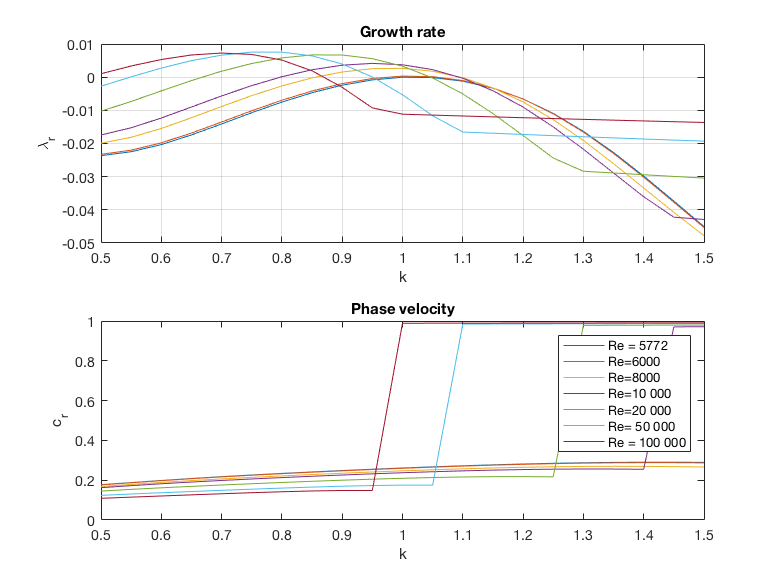
\includegraphics[width=.75\linewidth]{PlanePoiseuille_SigmaOmegaK.png}
$$
\caption{Taux de croissante $\lambda_r$ et vitesse de phase $c_r$ du mode le plus amplifié 
en fonction de $k$ pour $Re = 10^4$ et $M=0$ (noir), $M= 0.1$ (rouge), $M=0.6$ (bleu), et  $M=2$ (vert). }
\label{fig:branches}
\end{figure}


\begin{figure}
\begin{tabular}{cc}
\includegraphics[width=.49\linewidth]{BifDiagram_Exam2021.png}
&
\includegraphics[width=.49\linewidth]{PhasePortrait_Exam2021.png}
\\
$(a)$ & $(b)$ 
\end{tabular}
\caption{ ($a$) : Allure du diagramme de bifurcations pour l'équation \ref{eq:exo2a}.
%}
%\end{figure}
%\begin{figure}
%$$\includegraphics[width=.7\linewidth]{PhasePortrait_Exam2021.png}$$
%\caption{ 
$(b)$ :
Portrait de phase du système dynamique  \ref{eq:exo2b} avec le choix de paramètres. $r= -.9$; $A = 100$; $B=1$. Les lignes en rouge décrivent l'évolution vers le futur a partir d'une sélection de conditions initiales (correspondant aux cercles rouges); et les lignes pointillées roses leur évolution vers le passé.  }
\end{figure}




\end{document} 


%% EXAM 2020 :
\section{Instabilité d'un écoulement cisaillé à surface libre}

On considère un écoulement parallèle d'un liquide homogène de masse volumique $\rho$, défini par $\vec u = \bar{U}(y) \vec{e}_x
$ et associé à un champ de pression $\bar{P}(y)$, occupant l'espace $y \in [0,H]$. La position $y=0$ est un mur, et la position $y= \eta(x) = H$ une surface libre. La région $y>H$ est occupée par un gaz de masse volumique et viscosité négligeables, à la pression uniforme $P_a$.

La gravité est (sauf dans la partie D) supposée dirigée selon la verticale descendante : $\vec g = - g \vec e_y$ avec $g >0$.

Le liquide est supposé non non visqueux (sauf dans la partie E). 
 



 \begin{enumerate}
 
 \item { \bf Question préliminaire :} Montrez que le champ de pression $P(y)$ est un champ hydrostatique et donnez son expression.

{\bf A. Equations des perturbations (théorie non visqueuse)}

On étudie des petites perturbations à cet écoulement sous la forme modale suivante.
%\begin{equation}
$$
\left[ \begin{array}{c} u \\ v \\ p \\ \eta \end{array} \right] 
= 
\left[ \begin{array}{c} \bar{U}(y) \\ 0 \\ \bar{P}(y) \\ H \end{array} \right] 
+ 
\left[ \begin{array}{c} \hat{u}(y) \\ \hat{v}(y) \\ \hat{p}(y) \\ \hat{\eta} \end{array} \right] e^{i (k x -\omega t)} 
$$
%\end{equation}

\item Si $k$ est réel, expliquez la signification physique des parties réelles et imaginaires de $\omega$ .

\item 
A partir des équations d'Euler écrire 3 équations linéaires reliant $ \hat{u}(y)$, $\hat{v}(y)$ et $\hat{p}(y)$.

  \item Après avoir introduit une fonction de courant $\hat{\psi}$ (et justifié son existence), monter que ces équations peuvent se combiner pour aboutir à l'équation de Rayleigh (avec $c = \omega/k$):
  
 \begin{equation}
 (\bar{U} - c) (\partial_y^2 - k^2) \hat \psi + \bar{U}'' \hat \psi = 0
 \end{equation}
  
  \item 
  Ecrire deux conditions limites reliant respectivement $\hat{v}(H)$ à $\hat{\eta}$ et $\hat{p}(H)$ à $\hat{\eta}$
   
   \item Montrez que ces deux équations peuvent se combiner pour aboutir à l'expression suivante:
   
 \begin{equation}
  \left( U(H) - c\right)^2  {\left[ \frac{\partial \hat{\psi}}{\partial y} \right] }_{y=H}  - U'(H) \left( U(H) - c\right) \hat{\psi}(H) - g \hat{\psi}(H) = 0.
\end{equation}

\item Précisez également la condition limite vérifiée par $\hat{\psi}$ en $y=0$.


{\bf B. Cas particulier sans écoulement}

\item On suppose que $U(y) = 0$. Résolvez le problème et montrer qu'on retrouve la relation de dispersion classique des ondes de gravité en profondeur finie :
$\omega ^2 = g k \tanh (kH)$.

Dans ce cas particulier le problème est-il stable ou instable ?

 



{\bf C. Théorème de Rayleigh}

\item A partir de l'équation de Rayleigh, en supposant qu'il existe un mode instable vérifiant $c_i > 0$, démontrez l'identité suivante :

$$
 c_i \left\{ \int_{0}^{H} \frac{\bar{U}''(y)}{|\bar{U}(y)-c|^2} |\hat{\psi}(y)|^2 d y 
-  \frac{U'(H) }{|\bar{U}(H)-c|^2} |\hat{\psi}(H)|^2 + \frac{2 g (U(H) - c_r)  }{|\bar{U}(H)-c|^4} |\hat{\psi}(H)|^2
\right\} = 0.
$$

\item 

On suppose que $U'(y) >0$ et $U''(y) <0$ pour tout $y \in [0,H]$.
conclure que si $g=0$ il ne peux exister de mode instable. Ce résultat est-il en accord avec le théorème de Rayleigh ?


%\item Un théorème du à Howard (admis) permet de montrer que s'il existe un mode instable ($c_i >0$) alors la partie réelle de $c$ associée vérifie forcément $c_r  \in [\bar{U}_{min}, \bar{U}_{max}]$  ou $\bar{U}_{min}$ et 
%$\bar{U}_{max}$ sont les valeurs extrémales prises par $\bar{U}(y)$ sur l'intervalle $[0,H]$. En supposant toujours $U'(y) >0$ et $U''(y) <0$ pour tout $y \in [0,H]$, 
%que peut-on en conclure quand à l'existence possible de modes instables ?

%Cette conclusion est-elle en accord avec le théorème de Rayleigh ?


{\bf D. Solution dans le cas d'un cisaillement linéaire et d'une stratification inversée}

On suppose que le profil de vitesse est linéaire :
$\bar{U}(y) = V y/H$ 
Et que la gravité est maintenant orientée dans la direction $+y$ :

$\vec g = + g \vec e_y$ avec $g >0$. 

(En retournant les axes il s'agit donc d'un film liquide cisaillé "suspendu" sous une paroi horizontale).


\item Justifiez que l'équation de Rayleigh (1) est toujours valable et que la condition limite (2) doit être remplacée par :

 $$\left( V - c\right)^2  {\left[ \frac{\partial \hat{\psi}}{\partial y} \right] }_{y=H}  - \frac{V\left( V - c\right)}{H} \hat{\psi}(H) + g \hat{\psi}(H) = 0.
 $$

\item Montrez que les solutions du problème sont données par la relation de dispersion suivante  (où $\omega^{(rel)} = \omega - k V$ est la fréquence relative dans le repère se déplaçant à la vitesse $V$ de la surface libre): 
$$
\left[\omega^{(rel)}\right]^2 + \left[ \frac{V}{H} \omega^{(rel)} + g k \right] \tanh ( kH ) =0
$$

\item  Calculez le discriminant de cette equation et montrez que le problème est instable dans la limite des petites longueurs d'onde ($k\gg 1$).

Quel(s) effets non pris en compte dans l'analyse peuvent-ils modifier cette conclusion ?


\item 
Montrez que si $V>2 \sqrt{gH}$ les grandes longueurs d'ondes sont restabilisées par le cisaillement.
(Indice : on pourra raisonner graphiquement en comparant le comportement des fonctions $4kg$ et $(V/H)^2 \tanh(kH)$.)


{\bf E. Problème visqueux : résolution numérique}

\item A partir des équations de Navier-Stokes, écrire 3 équations linéaires 
reliant $ \hat{u}(y)$, $\hat{v}(y)$ et $\hat{p}(y)$.

\item Ecrire deux conditions-limites à vérifier en $y=0$ et trois conditions-limites à vérifier en $y=H$.
(Indice : la condition dynamique à la surface libre est à remplacer par la continuité des contraintes normales et tangentielles et fournit donc 2 équations). 
  
\item Montrez que le problème peut se mettre sous la forme matricielle $A \hat{q} = - i \omega B \hat{q}$ où $\hat{q} = [ \hat{u}, \hat{v}, \hat{p} , \hat{\eta} ]$. En déduire la structure d'un programme pour résoudre ce problème. 
  
\end{enumerate}



 
 


%\section{Le Brusselator}


%\subsection{Brusselator homogène}

%Le "Brusselator" est un système dynamique modélisant certaines réactions chimiques donnant lieu à des comportements complexes.
%Ce modèle correspond au système suivant :

%$$
%\frac{d x_1}{dt}  = −(\beta +1)x_1+x_1^2 x_2+\alpha,
%$$
%$$
%\frac{d x_2}{dt} = \beta x_1 - x_1^2 x_2;
%$$

%\clearpage

\section{Bifurcations d'une équation modèle}

On considère l'équation modèle suivante :
$$
\frac{ d x}{dt} = r x + A x^3 - x^5
$$

{\bf On considère dans les trois premières questions le le cas $A = 0$.}

\begin{enumerate}

\item Calculez les points d'équilibre de cette équation. Préciser le nombre de solutions en fonction du signe de $r$.

\item Etudiez (par la méthode de votre choix) la stabilité des points d'équilibre identifiés.

\item Tracez un diagramme des bifurcations. A quel type classique de bifurcation la situation étudiée ici est-elle apparentée ?

{\bf On considère pour les trois questions suivantes le cas $A = 1/2$.}

\item Calculez les points d'équilibre, et préciser leur nombre selon les cas $r<-1$, $-1<r<0$ et $r>0$.

\item  Etudiez (par la méthode de votre choix) la stabilité des points d'équilibre identifiés.

\item Tracez un diagramme des bifurcations. Préciser la nature des trois points de bifurcation observés sur ce diagramme.

\end{enumerate}






\end{document}



\item Donner la solution du système différentiel $\dot{\bf x} = A {\bf x}$, ${\bf x}(0) = {\bf x}_0$, pour les deux matrices suivantes : 
\begin{equation}
A = \left(
\begin{array}{cc}
a & 0 \\
0 & b
\end{array} \right) ; \qquad
A = \left(
\begin{array}{cc}
\sigma & -\omega \\
\omega & \sigma
\end{array} \right).
\end{equation}

%\item Soit le système différentiel $\dot{\bf x} = A {\bf x}$, $A = {\rm diag}(\lambda_1, \lambda_2)$. Tracer le portrait de phase pour $(\lambda_1, \lambda_2) = (Ð1,1)$ ; préciser le type du point fixe, et à quelle valeur propre correspond chaque direction propre.

%\item  Soit le système différentiel $\dot{\bf x} = A {\bf x}$, $A = {\rm diag}(\lambda_1, \lambda_2)$. Tracer le portrait de phase pour $(\lambda_1, \lambda_2) = (2,1)$ ; préciser le type du point fixe, et à quelle valeur propre correspond chaque direction propre.

%\item Les systèmes des deux questions précédentes sont-ils conservatifs ?

\item Donner la définition dÕun point fixe hyperbolique. Donner la définition de lÕéquivalence topologique de deux systèmes. Donner la condition de lÕéquivalence topologique dÕun système non linéaire et du système linéarisé en un point fixe.

\item On considère le système différentiel
\begin{eqnarray*}
\dot{x} = x (2 Ð x Ð y), \\
\dot{y} = y (3 Ð x Ð 2y).
\end{eqnarray*}
\begin{enumerate}
\item Déterminer les régions du plan $(x,y)$ o le flot défini par ce système est contractant ou dilatant. 
\item Déterminer les points fixes, leur stabilité, et leur type. 
\item Déterminer les directions propres pour chacun des points fixes. 
\item \'Ebaucher le portrait de phase au voisinage des points fixes. 
\item Compléter le portrait de phase, après avoir tracé le champ de vecteurs $(\dot{x}, \dot{y})$ sur les axes $x = 0$ et $y = 0$, sur les courbes telles que $\dot{x} = 0$ ou $\dot{y} = 0$, et déterminé les régions du plan o $\dot{x} > 0$ et $\dot{y} > 0$, $\dot{x} > 0$ et $\dot{y} < 0$, etc.
\end{enumerate}

\item On considère lÕoscillateur de DŸffing dissipatif 
\begin{equation}
\ddto{x}{t} + \epsilon \dto{x}{t} +  x - a x^3 = 0
\label{eq:0731bis}
\end{equation}
avec $\epsilon$ réel, $a >0$. Déterminer les points fixes dans lÕespace des phases. Déterminer le type du point fixe $(0, 0)$ selon la valeur de $\epsilon$.

%\item Quelle est la condition de stabilité linéaire dÕun point fixe $x_*$ d'un système différentiel $\dot{\bf x} = A {\bf x}$, ${\bf x} \in  \mathbb{R}^n$. Pour $n=2$, représenter les valeurs propres dans le plan complexe (a) pour $x_*$ stable, (b) pour $x_*$ instable.

\item Quelle est la condition de stabilité linéaire dÕun point fixe $x_*$ dÕune application ${\bf x}_{k+1} = f({\bf x}_k)$, ${\bf x} \in  \mathbb{R}^n$ ? Pour $n = 2$, représenter le spectre des valeurs propres dans le plan complexe (a) pour $x_*$ stable, (b) pour $x_*$ instable.

\item Déterminer les points fixes de lÕapplication 
\begin{equation}
x_{k+1} = x_k (1 + \mu - x_k),
\end{equation}
ainsi que leur stabilité, selon la valeur de $\mu$ réel.

\item \`A quelles condition un point fixe dÕune application est-il dit hyperbolique ? Pour quelles valeurs de $\mu$ les points fixes de lÕapplication ci-dessus sont-ils non hyperboliques ?

\item Déterminer les points périodiques de période minimale 2 de lÕapplication ci-dessus.


\end{enumerate}


\end{document} 

%%%%%%%%%%%%%%%%%%%%%%%%%%%%%%%%%%%%%%%%%%%%%%%%%%%%%%%%%%%%%%%%%%%%%%%%

NOM - Prénom :	4 mars 1998

Phénomènes non linéaires Ð Contr™le continu n¡ 2


6. Soit A = BBC[(AARHS2CO 2(a; b;c; d)) la matrice jacobienne dÕune application, calculée en un point fixe. Quelles inégalités les invariants de cette matrice doivent-ils vérifier pour que le point fixe soit un noeud stable ?

%%%%%%%%%%%%%%%%%%%%%%%%%%%%%%%%%%%%%%%%%%%%%%%%%%%%%%%%%%%%%%%%%%%%%%%%

NOM - Prénom :	Date : 18 mars 1998

Physique non linéaire Ð Contr™le continu n¡ 3

1. système O(x;¥) = f(x) : donner la forme normale et le diagramme de bifurcation dÕune bifurcation noeud-col.

2. système O(x;¥) = f(x) : donner la forme normale et le diagramme de bifurcation dÕune bifurcation fourche.

3. Soit le système O(x;¥) = mx Ð x2. Tracer le diagramme de bifurcation et préciser la nature de la bifurcation.

4. système O(w;¥) = f(w ) : Donner la forme normale et le diagramme de bifurcation dÕune bifurcation de Hopf.

5.Quel type de bifurcation lÕapplication xn+1 = mxn Ð xO(n;2)  subit-elle en m = 1.Tracer le diagramme de bifurcation. 

6. On considère une application xn+1 = f(xn) dont un point fixe perd son hyperbolicité pour m = 0 avec l = Ð1. A quel type de bifurcation peut-on sÕattendre ? Quelle condition f(x) doit-elle remplir pour quÕil en soit ainsi ?



%-----------------------------------------------------------------------
\section{Modèle de Lorenz de la convection de Rayleigh-Bénard} \label{sec:lorenz}

Le système de Lorenz est une modélisation extrême de la convection thermique de Rayleigh-Bénard, qui reproduit certains comportements observés expérimentalement, notamment l'apparition de rouleaux de convection au-delà d'une valeur critique du nombre de Rayleigh. Ce système s'écrit
\begin{eqnarray*}
\dot{x} &=& - P x + P y \\
\dot{y} &=& - y + r x - z x  \\
\dot{z} &=& - b z + x y,
\end{eqnarray*}

%où $x$ est une vitesse caractéristique, et $y$ et $z$ deux températures caractéristiques. $P$ est un nombre sans dimension analogue au nombre de Prandtl, $r$ correspond à un nombre de Rayleigh réduit, et $b$ correspond au nombre d'onde de la perturbation. On considère ici $r$ comme le paramètre variable, et les deux autre paramètres fixés aux valeurs classiques $P = 10$ et $b = 8/3$. 

\begin{enumerate}

\item Rappelez le lien entre ce système et la convection de Rayleigh-Bénard. Que représentent les 3 variables dynamiques $x$, $y$, $z$ ? A quoi correspondent les
paramètres $r$, $P$ et $b$ ?

Dans la suite on prendra les valeurs classiques $P = 10$ et $b = 8/3$ et on considèra $r$ comme paramètre de contrôle.

\item Etudiez la stabilité de la solution triviale $[x,y,z]$ = $[0,0,0]$. Montrez que celle-ci subit une bifurcation pour $r>1$. De quel type de bifurcation s'agit-il ?

\item Déterminer les points fixes non triviaux (notés $[x_p,y_p,z_p]$) du système apparaissant pour $r>1$. 

A quelles structures d'écoulement du problème de convection ces solutions correspondent-elles ?

\item Etudiez la stabilité linéaire des points fixes apparaissant pour $r>1$ en posant $[x,y,z] = [x_p,y_p,z_p] + \epsilon [\hat{x},\hat{y},\hat{z}] e^{\lambda t}$ 
avec $\epsilon \ll 1$.

Ecrire le polynôme caractéristique dont les racines sont les valeurs propres $\lambda$.

\item On admettra que le polynôme écrit précédemment a trois solutions, dont l'une est réelle et négative, et les deux autres complexes conjuguées de partie réelle négative lorsque $r < 24,74$ et positive lorsque $r>24.74$. 
A quel type de bifurcation peut-on s'attendre ?
   
\item Décrire en quelques mots la nature des solutions rencontrées pour $r>24.74$ et la signification physique de ces solutions pour le problème de convection.   

\end{enumerate}




\section{Instabilité d'une couche de mélange d'épaisseur nulle entre deux fluides non miscibles de même densité}


On étudie une couche de mélange (discontinuité de vitesse) entre deux fluides {\em non miscibles} 
mais {\em de masse volumique $\rho$ identique} .

Par exemple le demi-espace $y<0$ est rempli d'huile de parafine de vitesse $u =-U$ et le demi-espace $y>0$ est rempli d'alcool de vitesse
$ u = +U$ (deux liquides de densité sensiblement égale).

On note $\gamma$ la tension de surface ; les masses volumiques étant identiques {\em on pourra négliger la gravité }.

On souhaite étudier la stabilité linéaire de perturbations de longueur d'onde $\lambda = 2 \pi /k $ dans la direction $x$.
On suppose pour cela que l'interface est déplacée d'une amplitude $y = \eta(x,t) = C e^{i k x - i \omega t}+ c.c.$.

On admettra que la courbure d'une interface ainsi définie est donnée par $K \approx \partial^2 \eta/ \partial x^2$.
  



\begin{enumerate}

\item Montrez que des perturbations de nombre d'onde $k$ dans la direction $x$ sont gouvernées par la relation de dispersion suivante :
\begin{equation}
(k U + \omega)^2 + ( kU - \omega)^2 - \frac{\gamma}{\rho}  k^3 = 0
\end{equation} 

Vous utiliserez la démarche de votre choix pour établir cette relation mais veillerez à bien préciser et justifier les hypothèses faites dans la modélisation.

\item Représentez graphiquement $\omega_i$ en fonction de $k$ et $c_r = \omega_r/k$ en fonction de $k$.

\item Montrez qu'on a deux régimes différents correspondant à $k<k_c$ et $k>k_c$ avec $k_c = 2 \rho U^2 / \gamma$. 
Interprétez physiquement chacun de ces deux régimes.

\item Calculez la longueur d'onde $\lambda_{\max}$ correspondant au mode le plus amplifié, ainsi que le taux d'amplification $\omega_{i,max}$ correspondant.

\end{enumerate}


\section{Question de cours}

$$
\includegraphics[width=.55\linewidth]{FigureEcoulementsParalleles.png}
$$
\begin{enumerate}

\item
On considère 4 exemples d'écoulement parallèle d'un fluide incompressible représentés par les profils $(a)$, $(b)$, $(c)$, $(d)$ ci-dessus.
Pour chacun des cas, expliquez la signification physique de l'écoulement (dans quels contextes ou applications ce type d'écoulement est-il rencontré)
puis discutez ses propriétés de stabilité. A quel type d'instabilités peut-on s'attendre ?  Argumentez en vous basant sur les notions vues en cours (notamment les critères classiques de stabilité).


\end{enumerate}


\section{Evolution d'une population animale : étude de stabilité}

On étudie l'équation aux dérivées partielles suivante, gouvernant l'évolution de la fonction scalaire $\phi(x,t)$, définie dans l'intervalle $x\in [0,\infty]$ et $t\in [0,\infty]$ :

\begin{equation}
\frac{\partial \phi}{\partial t} + U \frac{\partial \phi}{\partial x} =  \sigma_0 \phi + \mu  \frac{\partial^2 \phi}{\partial x^2}  
\quad \quad 
\end{equation}


%associée aux conditions limites $\phi(0,t) = \phi(\infty,t) = 0$ et à la condition initiale $\phi(x,0) = \phi_0(x)$.

Ce modèle peut décrire par exemple l'évolution d'une colonie de micro-organismes dans une rivière en présence d'une source de nourriture $\sigma_0$ homogène, les bactéries subissant de plus une diffusion due à leurs déplacements aléatoires (modélisée par le coefficient de diffusion $\mu$) ainsi qu'une advection par le courant moyen (de vitesse uniforme $U$).

\begin{enumerate}

\item En recherchant des solutions modales en $x$ et $t$, (proportionnelles à $e^{i kx - i \omega t}$), écrire une relation de dispersion reliant $\omega$ et $k$.

\item En adoptant un point de vue {\em temporel}, ($k$ réel), exprimez $\omega$ en fonction de $k$. Quelles conditions sur les paramètres et sur $k$ conduisent à une instabilité ?

\item En étudiant le {\em point-selle} de cette relation de dispersion, précisez quelles conditions sur les paramètres conduisent à une instabilité convective ou absolue, respectivement.

({\em on admettra que ce point-selle vérifie la propriété de "chemin de descente la plus raide"}).

\item En considérant une population de micro-organismes initialement localisés au voisinage de $x=0$, comment se comporte la colonie dans les cas {\em absolu} et {\em convectif} ?


%\item Dans le cas on l'instabilité est convective, donnez les solutions $k^+(\omega)$ et k^-(\omega)$ du problème de stabilité spatiale ($\omega$ réel).


\end{enumerate}


